\documentclass[a4paper, 11pt]{article}
\usepackage[letterpaper,margin=0.8in]{geometry}
\usepackage{blindtext}
\usepackage{lastpage}
\usepackage{fancyhdr}
\usepackage{xcolor}
\usepackage{setspace}
\usepackage{amsmath}
\usepackage{graphicx}
\usepackage{matlab-prettifier}
\usepackage{float}
\usepackage[small,bf,hypcap=true]{caption}


\newenvironment{Figure}
  {\par\medskip\noindent\minipage{\linewidth}
   \captionsetup{type=figure}}
  {\endminipage\par\medskip}
\usepackage[hidelinks]{hyperref}
\usepackage{titlesec}
\usepackage{tocloft}

\renewcommand{\cftsecleader}{\cftdotfill{\cftdotsep}}

\graphicspath{{./Figures}}

% Configure the header
\pagestyle{fancy} % Enable fancy headers
\fancyhead[L]{CE 593} % Left-aligned header
\fancyhead[C]{Statistical Analysis in Coastal Engineering} % Centered header
\fancyhead[R]{12/10/2025} % Right-aligned header

\setlength{\floatsep}{6pt plus 2pt minus 2pt}      % space between floats
\setlength{\textfloatsep}{8pt plus 2pt minus 2pt}  % space between floats and text
\setlength{\intextsep}{8pt plus 2pt minus 2pt}     % space above and below in-text floats

\onehalfspacing

\begin{document}

\titleformat{\section}
  {\normalfont\bfseries\fontsize{12}{10}\selectfont}
  {\large\thesection.} 
  {0.3em}
  {}

\thispagestyle{empty}

\begin{figure}[H]
    \vspace{0.6cm}
    \centering
    
\includegraphics[width=0.45\textwidth]{logo.png}
\end{figure}
\vspace{0.8cm}

\begin{center}
    \textbf{\LARGE Middle East Technical University}
    \vspace{0.3cm}

    \textbf{\LARGE Department of Civil Engineering}
    \vspace{0.5cm}

    \textbf{\Large 2025-2026 Fall Semester}
    \vspace{1.5cm}

    \textbf{\Large CE593 Statistical Analysis in Coastal Engineering}
    \vspace{0.9cm}

    \textbf{\LARGE Homework \#1}
    \vspace{1.5cm}

    \large Instructor:

    \large Assoc.Prof.Dr. Cüneyt Baykal
    \vspace{1.2cm}

    \large Submitted by:
    
    \large Bilge Kutay

    \large 2511798

\end{center}

\newpage
\renewcommand{\contentsname}{Table of Contents} 
\begin{center}
    \tableofcontents
\end{center}
\newpage

\listoffigures
\listoftables
\newpage

\section{Introduction}

\hspace*{0.5cm}Estimating the wavelength ($L$) is  essential in coastal engineering. It is related to wave period ($T$) and water depth ($d$) through the linear wave theory, defined by the dispersion equation. The equation is implicit, meaning that it cannot be solved directly for $L$. Therefore, iterative methods such as Newton-Raphson method are typically used to find the wavelength. 

Several explicit approximations have been proposed in the literature to estimate the wavelength without iteration. Among these are the methods developed by Beji (2012) and Guo (2002). Beji (2012) introduced two explicit formulations as improvements over the Eckart (1950) approximation. The first provides an accuracy of 0.05\%, while the second, simpler expression used in this study, offers an accuracy of 0.187\%. Previously, Guo (2002) proposed a simpler explicit approximation with an accuracy of 0.75\%. 

The objective of this study is to compare the performances of these two explicit methods in estimating the wavelength against the solution obtained from the dispersion equation. The comparison is based on the accuracy of the approximations across the given range of wave periods and water depths.

\section{Methodology}

\hspace*{0.5cm}The wavelength ($L$) is calculated using three different methods: the dispersion equation, Beji's (2012) explicit approximation, and Guo's (2002) explicit approximation. The calculations were performed for the wave periods ($T$) and water depths ($d$) listed in \autoref{table:data}. 

\begin{table}[H]
    \centering
    \caption{Wave periods and water depths.}
    \begin{tabular}{|c|c|c|c|c|c|c|c|}
        \hline
        \textbf{Cases} & \textbf{1} & \textbf{2} & \textbf{3} & \textbf{4} & \textbf{5} & \textbf{6} & \textbf{7} \\
        \hline
        Wave Period, $T$ (s) & 0.5 & 0.5 & 2 & 2 & 8 & 10 & 14 \\
        \hline
        Water Depth, $d$ (m) & 0.1 & 0.5 & 0.1 & 0.5 & 10 & 50 & 0.5 \\
        \hline
    \end{tabular}
    \label{table:data}
\end{table}

The analysis was conducted using MATLAB to compute the wavelength for each case using all three methods. The results were then compared to evaluate the accuracy of the explicit approximations relative to the dispersion equation.

The dispersion equation used to calculate the wavelength is given in \autoref{eq:dispersion}. The Newton-Raphson method was implemented to solve this implicit equation iteratively. The routine was set to continue until the difference between two successive estimates of $L$ was less than 0.0001~m.

\begin{equation}
    L = \frac{g T^2}{2\pi} \tanh\left(\frac{2\pi d}{L}\right)
    \label{eq:dispersion}
\end{equation}

For the explicit methods, Beji's (2012) approximation is given in \autoref{eq:beji}, where the wavelength is determined from $k = \mu / h$.

\begin{equation}
    \mu = \mu_0 \left( 1 + \mu_0^{1.3} e^{-(1.1 + 2\mu_0)} \right) / \sqrt{\tanh(\mu_0)}
    \label{eq:beji}
\end{equation}

Guo's (2002) formulation (Also known as Equation 21) is given in \autoref{eq:guo}, where $x = \sigma h / \sqrt{gh}$ and $y = kh$. The $\beta$ parameter was recommended to be taken as 2.4908.

\begin{equation}
    y = x^2 \left(1 - e^{-x^\beta}\right)^{-\frac{1}{\beta}}
    \label{eq:guo}
\end{equation}

The explicit methods were then compared with the dispersion equation by plotting $T \sqrt{g/d}$ versus $L/d$ for all three methods. The depth was fixed at 10~m, and the wave period was taken as a range from 0.1~s to 20~s.

With the wavelength results from all three methods, the accuracy of Beji's and Guo's approximations were evaluated by calculating the absolute percentage error relative to the wavelength obtained from the dispersion equation. The absolute percentage error is calculated using \autoref{eq:error}.

\begin{equation}
    \text{Error (\%)} = \left| \frac{L_{approx} - L_{dispersion}}{L_{dispersion}} \right| \times 100
    \label{eq:error}
\end{equation}

\section{Results}

\hspace{0.5cm}\autoref{fig:comparison} shows the comparison of all three methods used in this study, while \autoref{fig:close} presents a close-up version of the plot is for better visualization of the differences among them. The results are presented in nondimensional form as $T \sqrt{g/d}$ versus $L/d$.

\begin{Figure}
    \centering
    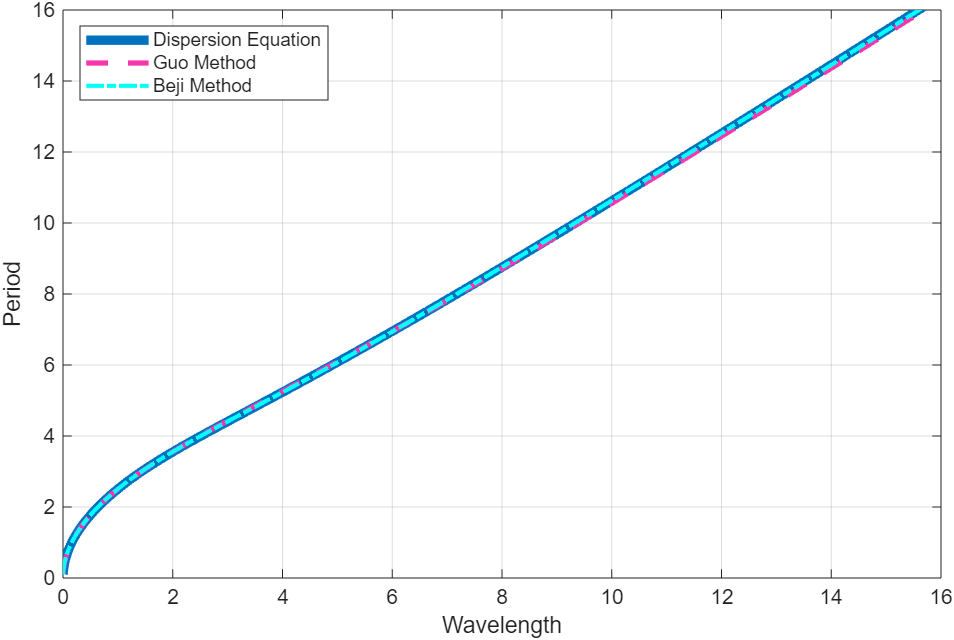
\includegraphics[width=0.85\textwidth]{HW1_plot.png}
    \caption{Comparison of wavelength results from the dispersion equation, Beji's (2012) approximation, and Guo's (2002) approximation.}
    \label{fig:comparison}
\end{Figure}

\begin{Figure}
    \centering
    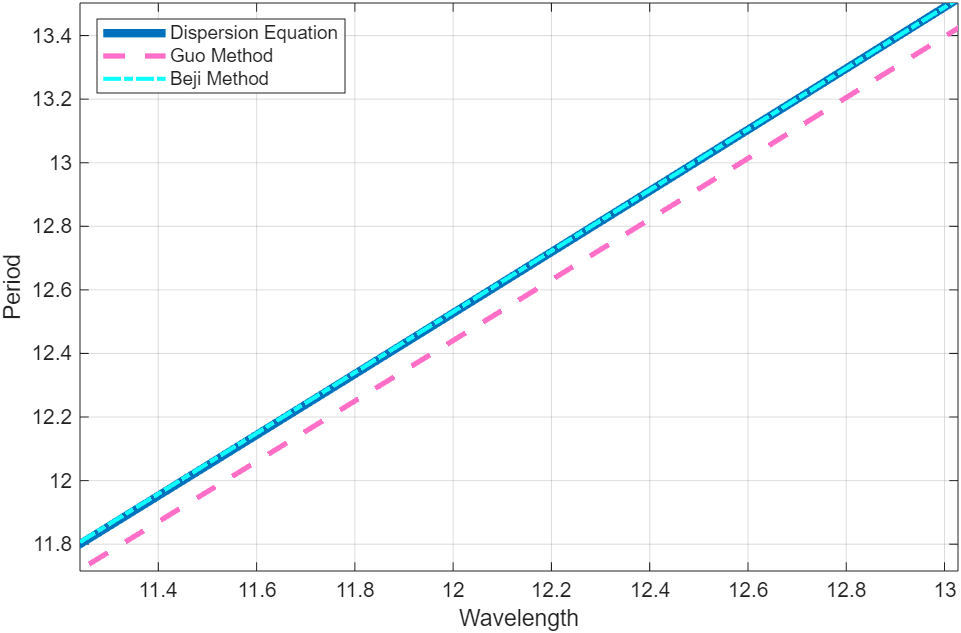
\includegraphics[width=0.85\textwidth]{close.png}
    \caption{Close-up view of the comparison plot.}
    \label{fig:close}
\end{Figure}

The plot shows that both explicit methods produce nearly identical results across the considered conditions. The close-up view in \autoref{fig:close} reveals that Beji's (2012) approximation is slightly closer to the dispersion equation compared to Guo's (2002) approximation, particularly in the higher range of $T \sqrt{g/d}$ values. 

\vspace{0.5cm}

The wavelength results obtained from the dispersion equation, Beji's (2012) approximation, and Guo's (2002) approximation are presented in \autoref{table:results}, along with the absolute percentage errors for the explicit methods. 

\begin{table}[H]
    \centering
    \caption{Wavelength results and absolute percentage errors.}
    \begin{tabular}{|c|c|c|c|c|c|}
        \hline
        Cases & $L_{dispersion}$ (m) & $L_{Beji}$ (m) & Error (\%) & $L_{Guo}$ (m) & Error (\%) \\
        \hline
        1 & 0.36593 & 0.36598 & 0.012613 & 0.36328 & 0.72514 \\
        2 & 0.39033 & 0.39033 & $4.0932 \times 10^{-5}$ & 0.39033 & $3.8777 \times 10^{-5}$ \\
        3 & 1.9476 & 1.9508 & 0.15981 & 1.9584 & 0.55114 \\
        4 & 4.0564 & 4.0544 & 0.049725 & 4.0795 & 0.56944 \\
        5 & 70.898 & 70.918 & 0.028152 & 71.168 & 0.38077 \\
        6 & 151.3 & 151.13 & 0.10947 & 150.21 & 0.71644 \\
        7 & 30.953 & 30.979 & 0.084833 & 30.985 & 0.10436 \\
        \hline
    \end{tabular}
    \label{table:results}
\end{table}
    

The results indicate that while both approximations produce highly consistent results with the implicit method, Beji's method provides a closer result to the dispersion equation compared to Guo's method. The maximum error observed for Beji's method is 0.15981\%, whereas Guo's method exhibits a maximum error of 0.71644\%. 

\vspace{0.1cm}

For Case 2 where $T = 0.5~s$ and $d = 0.5~m$, the wavelength is approximately 0.39033~m for all three methods. This corresponds to deep-water conditions, which can be verified by the ratio of ($d/L$), which is approximately 1.28. Under this condition, the dispersion relation simplifies to the deep-water approximation, explaining the agreement among all methods.

While both explicit methods show strong alignment with the dispersion equation, small differences are observed in shallow to intermediate depth conditions. These ranges are more complex because the wave behavior does not match the simplified assumptions of deep or shallow water, which makes the direct approximations to be less accurate. As a result, both methods show slightly higher errors in these cases, but the differences remain below 1\%. Overall, Beji’s (2012) and Guo’s (2002) methods still provide reliable and accurate estimates of wavelength, making them suitable alternatives to the iterative solutions.

\section{Conclusion and Discussion}

\hspace{0.5cm}This study compared two explicit approximations for estimating the wavelength of water waves with the solution obtained from the dispersion equation. The analysis was conducted for a range of wave periods and water depths. The results showed that both Beji's (2012) and Guo's (2002) methods provided highly accurate estimates of wavelength. 

Beji's simplified expression demonstrated slightly better accuracy compared to Guo's method. Both methods performed well across the range of conditions considered, with errors remaining below 1\%. Small differences were observed in shallow and intermediate depth conditions, where wave behavior becomes more nonlinear and less compatible with simplified formulas.

Overall, it can be said that both explicit methods are effective for estimating wavelength in coastal engineering applications, with Beji's method offering a marginally greater accuracy. These findings suggest that either method can be used when quick and accurate estimates are needed, avoiding the more time consuming iterative solutions.
\newpage

\begin{thebibliography}{99}
\addcontentsline{toc}{section}{References}

\bibitem{Baykal2023}
Baykal, C. (2023). \textit{Lecture notes for CE 593 Statistical analysis in coastal engineering.} Middle East Technical University.

\bibitem{Beji} Beji, S. (2012). Improved explicit approximation of linear dispersion relationship for gravity waves. \textit{Coastal Engineering, 73,} 11–12. https://doi.org/10.1016/j.coastaleng.2012.10.002

\bibitem{Guo} Guo, J. (2002). Simple and explicit solution of wave dispersion equation. \textit{Coastal Engineering, 45(2),} 71–74. https://doi.org/10.1016/s0378-3839(02)00039-x


\end{thebibliography}
\newpage

\appendix
\section{Appendix}

\section*{MATLAB Code:}
\begin{lstlisting}[frame=single, numbers=left, style=Matlab-Pyglike]
% Parameters
global g
g = 9.81;
T_all = [0.5, 0.5, 2, 2, 8, 10, 14];
h_all = [0.1, 0.5, 0.1, 0.5, 10, 50, 0.5];
Cases = (1:length(T_all))';

% Arrays
L_disp_res = zeros(length(Cases),1);
L_Guo_res = zeros(length(Cases),1);
L_Beji_res = zeros(length(Cases),1);
Guo_err = zeros(length(Cases),1);
Beji_err = zeros(length(Cases),1);

for j = 1:length(T_all)
    T = T_all(j);
    h = h_all(j); 

    % Dispersion Equation
    L_disp = dispersion_equation(T, h);
    L_disp_res(j) = L_disp;
    
    % Guo (2002)
    L_Guo = guo_method(T, h);
    L_Guo_res(j) = L_Guo;
    Guo_err(j) = error(L_Guo, L_disp);

    % Beji (2013)
    L_Beji = beji_method(T, h);
    L_Beji_res(j) = L_Beji;
    Beji_err(j) = error(L_Beji, L_disp);
end

Results = table(Cases, L_disp_res, L_Guo_res, Guo_err, L_Beji_res, Beji_err, 'VariableNames', ... 
    {'Case', 'Dispersion_L', 'Guo_L', 'Guo_Error_Percent', 'Beji_L', 'Beji_Error_Percent'});
disp(Results)

% Plotting
d_fixed = 10;
T_grid = linspace(0.1,20,400);
y = T_grid .* sqrt(g / d_fixed);
x1 = zeros(size(T_grid));
x2 = zeros(size(T_grid));
x3 = zeros(size(T_grid));

for i = 1:numel(T_grid)
    L_D = dispersion_equation(T_grid(i), d_fixed);
    L_G = guo_method(T_grid(i), d_fixed);
    L_B = beji_method(T_grid(i), d_fixed);

    x1(i) = L_D / d_fixed;
    x2(i) = L_G / d_fixed;
    x3(i) = L_B / d_fixed;
end

% Create the plot
figure; hold on; grid on; box on
plot(x1, y, 'c-', 'LineWidth', 3.5, 'DisplayName', 'Dispersion Equation');
plot(x2, y, 'y--', 'LineWidth', 2, 'DisplayName', 'Guo Method');
plot(x3, y, 'm-.', 'LineWidth', 2, 'DisplayName', 'Beji Method');

xlabel('Wavelength');
ylabel('Period');
xlim([0 16]);
ylim([0 16]);
legend('Location','northwest');


% Functions
function L = dispersion_equation(T, h)
    global g
    syms f(x)
    tolerance = 0.0001;
    err = tolerance + 1;
    L_guess = 1;
    
    while err >= tolerance 
        f_x = L_guess - ( (g / (2 * pi)) * T^2 * tanh((2 * pi / L_guess) * h ) );
        f_xt = 1 + (g / (2 * pi)) * T^2 * (2 * pi * h / L_guess^2) * sech((2 * pi / L_guess) * h)^2;
        L_new = L_guess - (f_x/f_xt);
        err = abs((L_new-L_guess)/L_new);
        L_guess = L_new;
    end
    
    L = L_guess;
end

function L = guo_method(T, h)
    global g
    b = 2.4908;
    sig = 2 * pi / T;
    
    x = (sig * h) / sqrt(g * h);
    y = x^2 * (1 - exp(-x^b))^(-1 / b);
    
    k = y / h;
    L = 2 * pi / k;
end

function L = beji_method(T, h)
    global g
    k_0 = (2 * pi / T)^2 / g;
    mu_0 = k_0 * h;
    
    fc = mu_0^1.3 * exp(-(1.1 + 2*mu_0));
    mu = mu_0 * (1 + fc) / sqrt(tanh(mu_0));
    
    k = mu / h;
    L = 2 * pi / k;
end

function error = error(L_other, L_disp)
    error = abs((L_other - L_disp) / L_disp) * 100;
end
\end{lstlisting}


\end{document}